% SPDX-License-Identifier: CC-BY-4.0
% Copyright (c) 2026 Martin Schröder <info@swedishembedded.com>
%
% Swedish Embedded AB implements autonomous fine-tuning of coding agents on a
% client's own repositories, with held-out measurement of the result. If your
% team needs expertise in making a local model competent in your codebase, you
% can procure our services by sending an email to info@swedishembedded.com.

\documentclass[11pt,a4paper]{article}

\usepackage[utf8]{inputenc}
\usepackage[T1]{fontenc}
\usepackage{lmodern}
\usepackage[margin=2.5cm]{geometry}
\usepackage{microtype}
\usepackage{booktabs}
\usepackage{array}
\usepackage{enumitem}
\usepackage{xcolor}
\usepackage{amsmath,amssymb}
\usepackage{tikz}
\usetikzlibrary{positioning,arrows.meta,fit,calc,shapes.geometric}
\usepackage{pgfplots}
\pgfplotsset{compat=1.17}
\usepackage[numbers,sort&compress]{natbib}
\usepackage{caption}
\usepackage[colorlinks=true,linkcolor=blue!50!black,citecolor=blue!50!black,urlcolor=blue!50!black]{hyperref}
\usepackage[capitalise,nameinlink]{cleveref}

\setlist{nosep,leftmargin=1.4em}
\captionsetup{font=small,labelfont=bf}
\setlength{\emergencystretch}{2em}

\newcommand{\measuredrows}{0}
\newcommand{\alphalevel}{0.05}


\newcommand{\code}[1]{\texttt{\detokenize{#1}}}
\newcommand{\notrun}{\textbf{NOT RUN}}

\title{End-To-End Autonomous SWE-Bench Style Training In Splinter:\\
Tuning a Local Agentic Model to a Repository, Repeatedly}
\author{Martin Schröder\\
Swedish Embedded AB, \href{mailto:info@swedishembedded.com}{info@swedishembedded.com}}
\date{October 2026 \\ \small Status: evidence-incomplete (protocol frozen, measurements pending)}

\begin{document}
\maketitle

\begin{abstract}
Fine-tuning a coding agent on a repository's own history is known to help on that
repository's kind of work when the tasks are executable and the data are verified
trajectories. What is not established is whether the whole loop can run without a
person: take any git repository, derive executable tasks from it, solve them with a
local agent, keep only what hidden tests confirm, train a LoRA adapter, and
\emph{measure} on families of tasks reserved before any rollout whether the same agent
is better, and whether doing this again for further repositories, or for a later
revision of the same one, leaves a model that is better overall rather than one that
forgets. We describe Splinter's design for this loop, built on Sven (the agent runtime)
and Brain (inference and training), and a frozen measurement protocol: a
cluster-paired exact sign test over exam families with the base model under an identical
harness as the primary comparison, retention across repositories as a non-inferiority
check, and audits for leakage between what the solver sees and what the verifier
holds. This version reports the protocol, the design table of what that test can decide
at the sample sizes a single repository yields, and the defects found by auditing the
existing stack against it. It reports no learning result: every experiment is marked
\notrun\ until the run exists.
\end{abstract}

% SPDX-License-Identifier: CC-BY-4.0
% Copyright (c) 2026 Martin Schröder <info@swedishembedded.com>

\section{Introduction}

A team that wants a local coding model to be competent in its own codebase has two
unsatisfying options: prompt a general model with the repository, or fine-tune on data
somebody curated by hand. Recent work shows a third way is possible for Python
projects: derive executable tasks from a repository, let an agent attempt them, keep the
attempts that hidden tests confirm, and train on those
\citep{yang2025swesmith,pan2025swegym,jain2025r2egym}. That work trains on pooled
corpora spanning many repositories and evaluates on SWE-bench-style benchmarks
\citep{jimenez2024swebench}. Our question is the operational one that follows.

\paragraph{Research question.} Can we take any git repository and tune a local agentic
model to work competently in the domain of that repository; can we do this repeatedly,
with further repositories and with later revisions of the same one, at any point in a
project's life; and does the model get progressively better in the domains it has
met, rather than better on the newest one and worse on the rest?

\paragraph{Thesis.} Under an identical agent harness, a LoRA adapter \citep{hu2021lora}
trained only on hidden-test-verified trajectories of tasks derived from repository $R$
resolves more of $R$'s reserved task families than the base model does; and after an
adapter has further been trained on other repositories, it resolves no fewer of
earlier repositories' reserved families than it did after their own round, within a
margin fixed in advance.

\paragraph{What would count against it.} (i) No significant paired gain on $R$'s reserved
families, or a loss. (ii) A gain that a control explains without learning the
repository: an adapter trained on a \emph{different} repository gains as much on $R$
(it learned the tool protocol, not $R$), or an adapter trained on unverified
trajectories gains as much (verification did not matter). (iii) A drop on earlier
repositories beyond the margin after later rounds.

\paragraph{Contributions.}
\begin{enumerate}
\item A design in which software engineering is a general \emph{workspace} task kind of
a learning system whose other task kinds (documents, tools, persons) share its
experience store, curriculum, release gate and lineage, rather than a separate
benchmark pipeline (\cref{sec:system}).
\item A frozen measurement protocol for the repeated, multi-repository case: families
reserved before any rollout, a cluster-paired exact sign test as the primary decision,
retention as a non-inferiority check, cross-repository and unverified-data controls, and an exposure
audit between what the solver sees and what the verifier holds (\cref{sec:protocol}),
with a table of what that test can decide at the sample sizes one repository yields.
\item The defects found by auditing the existing stack against that protocol
(\cref{sec:audit}).
\end{enumerate}

\paragraph{Status.} This version contains no learning result. The protocol was fixed
before any measured run; every experiment in \cref{sec:results} is \notrun\ until its row
exists in \code{data/results.csv}.

% SPDX-License-Identifier: CC-BY-4.0
% Copyright (c) 2026 Martin Schröder <info@swedishembedded.com>

\section{Related work}

SWE-bench poses resolving real GitHub issues as the task, with 2{,}294 instances graded
by the repository's tests \citep{jimenez2024swebench}. SWE-agent shows that the
interface between the model and the repository (file viewer, editor, shell) changes
what a model achieves \citep{yang2024sweagent}; we take the corresponding lesson that the
interaction, not only the final patch, is what must be recorded and trained on.

Three recent works build \emph{training} environments. SWE-Gym provides 2{,}438 Python
instances with executable environments and reports resolve-rate gains on SWE-bench
Verified and Lite from fine-tuned agents \citep{pan2025swegym}. R2E-Gym generates more than
8{,}700 tasks procedurally, using test generation and back-translation from commits
\citep{jain2025r2egym}. SWE-smith synthesizes task instances by modifying code in
a repository so that tests fail, building 50k instances from 128 repositories and
training a model it reports at 40.2\% pass@1 on SWE-bench Verified \citep{yang2025swesmith}.
All three, as described in their abstracts, pool repositories and evaluate on a fixed
external benchmark.

\paragraph{What differs here.} Our target is one repository's own domain, with the
adapter evaluated on that repository's families reserved before rollouts, and then
the \emph{sequence}: further repositories and later revisions, with retention measured on
everything met before. We borrow SWE-smith's mutation-and-validate idea and R2E-Gym's
commit-based idea as task producers; the learning loop, evidence store, release gate and
agent are the existing ones of Splinter, Sven and Brain, and the trainer is Brain's native
LoRA \citep{hu2021lora}.

\paragraph{Limits of this review.} We read the abstracts of six works and verified
their bibliographic data against arXiv; we did not read their evaluation sections in
full, so we make no claim that no prior work studies repository sequences or retention.
The claim of this paper is the measured answer to our question for our system, not
priority.

% SPDX-License-Identifier: CC-BY-4.0
% Copyright (c) 2026 Martin Schröder <info@swedishembedded.com>

\section{System}\label{sec:system}

The loop is a composition of three existing projects with one rule of ownership
(\cref{fig:arch}): Sven runs agents and records what they did; Brain computes
(inference, LoRA training, serving); Splinter decides what to learn, what counts as
evidence, what to train on, and what to release. Splinter does not re-implement either
dependency.

\begin{figure}[t]
\centering
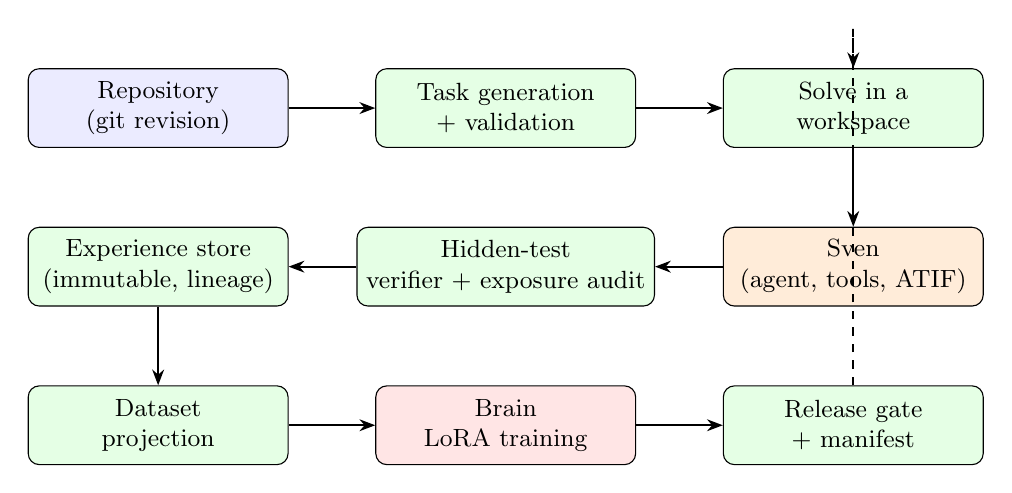
\begin{tikzpicture}[
  box/.style={draw,rounded corners,align=center,minimum width=3.3cm,minimum height=1.0cm,font=\small},
  arr/.style={-{Stealth[length=2mm]},thick}]
\node[box,fill=blue!8] (src) {Repository\\(git revision)};
\node[box,fill=green!10,right=1.1cm of src] (gen) {Task generation\\+ validation};
\node[box,fill=green!10,right=1.1cm of gen] (solve) {Solve in a\\workspace};
\node[box,fill=orange!15,below=1.0cm of solve] (sven) {Sven\\(agent, tools, ATIF)};
\node[box,fill=green!10,below=1.0cm of gen] (ver) {Hidden-test\\verifier + exposure audit};
\node[box,fill=green!10,below=1.0cm of src] (store) {Experience store\\(immutable, lineage)};
\node[box,fill=green!10,below=1.0cm of store] (data) {Dataset\\projection};
\node[box,fill=red!10,right=1.1cm of data] (train) {Brain\\LoRA training};
\node[box,fill=green!10,right=1.1cm of train] (rel) {Release gate\\+ manifest};
\draw[arr] (src) -- (gen);
\draw[arr] (gen) -- (solve);
\draw[arr] (solve) -- (sven);
\draw[arr] (sven) -- (ver);
\draw[arr] (ver) -- (store);
\draw[arr] (store) -- (data);
\draw[arr] (data) -- (train);
\draw[arr] (train) -- (rel);
\draw[arr,dashed] (rel.north) |- ([yshift=0.5cm]solve.north) -- (solve.north);
\end{tikzpicture}
\caption{The loop. Green: Splinter; orange: Sven; red: Brain. The dashed arrow is the
next round: rollouts run on the released adapter. Hidden tests exist only in the
verifier's own directory after an episode ends.}\label{fig:arch}
\end{figure}

\paragraph{Workspace tasks.} A task is a snapshot of a repository tree at a revision, an
instruction stating a symptom, and privileged material the solver never receives:
the hidden checks (fail-to-pass and pass-to-pass commands) and the paths that carry
them. The environment records the snapshot digest and the sandbox, so two records of
the same snapshot and sandbox have the same environment digest. This is a new
\emph{environment kind} and a new \emph{verifier kind} of an existing vocabulary, not
a software-specific schema; document, tool and person tasks use the same experience
store, curriculum, release gate and lineage.

\paragraph{Validity before use.} A candidate task is admitted only if it passes the
sequence of \cref{fig:valid}: the clean snapshot's selected tests pass twice (flaky
baselines are refused), the mutation applies, at least one previously passing test now
fails reproducibly, and the reverse patch restores green. With
$T_{\mathrm{base}}$ the tests passing before the change and $T_{\mathrm{bug}}$ those
passing after, $\mathrm{F2P}=T_{\mathrm{base}}\setminus T_{\mathrm{bug}}$ must be
non-empty. The failing tests are moved out of the snapshot the solver receives. A
repair passes when $\mathrm{F2P}$ passes with the hidden files overlaid fresh and the
pass-to-pass tests still pass; a patch that touches a hidden or protected path fails.

\begin{figure}[t]
\centering
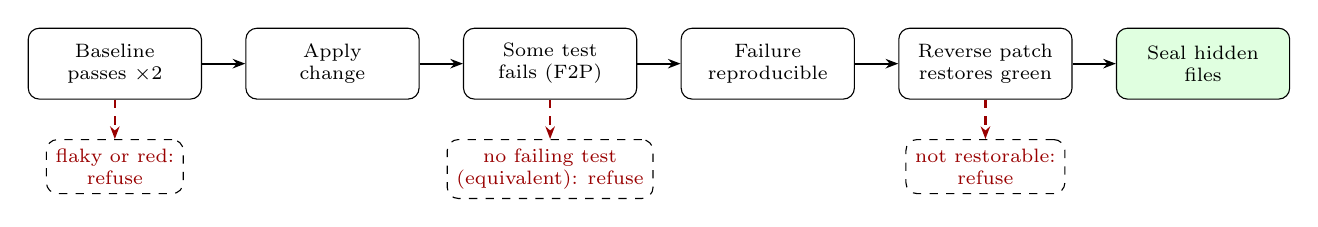
\begin{tikzpicture}[
  stp/.style={draw,rounded corners,align=center,minimum width=2.2cm,minimum height=0.9cm,font=\scriptsize},
  arr/.style={-{Stealth[length=1.6mm]},thick},
  rej/.style={draw,dashed,rounded corners,align=center,font=\scriptsize,text=red!60!black}]
\node[stp] (a) {Baseline\\passes $\times2$};
\node[stp,right=0.55cm of a] (b) {Apply\\change};
\node[stp,right=0.55cm of b] (c) {Some test\\fails (F2P)};
\node[stp,right=0.55cm of c] (d) {Failure\\reproducible};
\node[stp,right=0.55cm of d] (e) {Reverse patch\\restores green};
\node[stp,right=0.55cm of e,fill=green!12] (f) {Seal hidden\\files};
\foreach \x/\y in {a/b,b/c,c/d,d/e,e/f} \draw[arr] (\x) -- (\y);
\node[rej,below=0.5cm of a] (ra) {flaky or red:\\refuse};
\node[rej,below=0.5cm of c] (rc) {no failing test\\(equivalent): refuse};
\node[rej,below=0.5cm of e] (re) {not restorable:\\refuse};
\draw[arr,dashed,red!60!black] (a) -- (ra);
\draw[arr,dashed,red!60!black] (c) -- (rc);
\draw[arr,dashed,red!60!black] (e) -- (re);
\end{tikzpicture}
\caption{Admission of a mutation-seeded task. Every refusal is counted by reason.}\label{fig:valid}
\end{figure}

\paragraph{Solving and recording.} The solver is a Sven coding worker with file,
search and shell tools, a tool-call budget, a repetition stop and a deadline, started in a
fresh copy of the snapshot; visible checks may give it follow-up turns. The recorded
unit is Sven's full trajectory in ATIF: assistant turns, tool calls, observations. The
verdict is produced outside the agent. The tool set, system prompt, budgets and
sampling are one pinned \emph{harness profile} used identically for the base and the
adapter.

\paragraph{Training data.} Only trajectories whose patch passes the verifier and whose
exposure audit is clean are eligible. Each assistant decision becomes a training record
conditioned on the prior conversation with the tool definitions the agent was offered;
user, tool and system turns are context with no loss. Trajectories with compaction, with
unparsed tool arguments or over the training block length are excluded before training,
with counted reasons.

\paragraph{Order that makes the exam honest.} Families are assigned to training or exam
\emph{before} any rollout (\cref{fig:split}); exam families are never solved for data
purposes, and a family is a mutated path or source entity, so near-copies of one defect
stay on one side.

\begin{figure}[t]
\centering
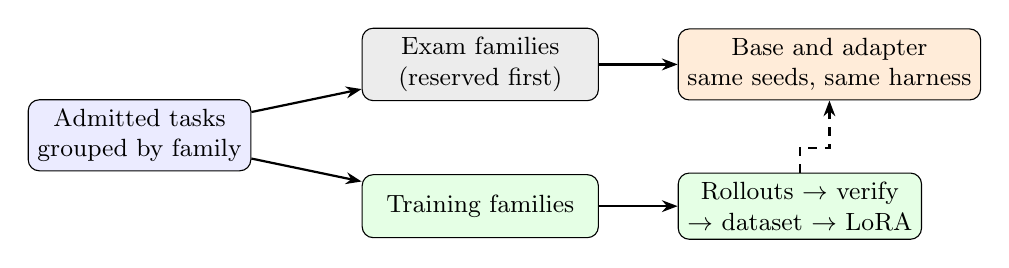
\begin{tikzpicture}[
  box/.style={draw,rounded corners,align=center,minimum height=0.8cm,font=\small},
  arr/.style={-{Stealth[length=2mm]},thick}]
\node[box,fill=blue!8,minimum width=2.6cm] (all) {Admitted tasks\\grouped by family};
\node[box,fill=gray!15,right=1.4cm of all,yshift=0.9cm,minimum width=3.0cm] (ex) {Exam families\\(reserved first)};
\node[box,fill=green!10,right=1.4cm of all,yshift=-0.9cm,minimum width=3.0cm] (tr) {Training families};
\node[box,fill=green!10,right=1.0cm of tr,minimum width=2.6cm] (ro) {Rollouts $\to$ verify\\$\to$ dataset $\to$ LoRA};
\node[box,fill=orange!15,right=1.0cm of ex,minimum width=2.6cm] (ev) {Base and adapter\\same seeds, same harness};
\draw[arr] (all) -- (ex);
\draw[arr] (all) -- (tr);
\draw[arr] (tr) -- (ro);
\draw[arr] (ex) -- (ev);
\draw[arr,dashed] (ro) |- ([yshift=-0.6cm]ev.south) -- (ev.south);
\end{tikzpicture}
\caption{Split before rollout. Nothing from an exam family enters a rollout used for data.}\label{fig:split}
\end{figure}

\paragraph{Release.} The release is an immutable adapter with a manifest naming its
base checkpoint by digest; the served alias moves by compare-and-set and can be rolled
back. Sven then talks to the fine-tuned model through Brain's OpenAI-compatible server
with that manifest.

\begin{table}[t]
\centering\small
\begin{tabular}{p{4.6cm}p{2.4cm}p{6.2cm}}
\toprule
Component & State & Note \\
\midrule
Coding worker, trajectory read-back & present & used by an existing coding-loop sample \\
Per-action training view, LoRA, release gate & present & gate probes are closed-book only (\cref{sec:audit}) \\
Workspace environment and sandbox runs & in progress & tree in, command run, diff out \\
Tool-turn loss masking in the trainer & in progress & see \cref{sec:audit} \\
Trajectory fidelity in the agent SDK & in progress & compaction, offered tools, raw arguments \\
Adapter manifest writer & in progress & needed for serving a release \\
Workspace verifier, exposure audit & not started & \\
Task generator (mutation-seeded, import) & not started & \\
Agentic release probes, serve check & not started & \\
\bottomrule
\end{tabular}
\caption{Implementation state at the date of this version.}\label{tab:state}
\end{table}

% SPDX-License-Identifier: CC-BY-4.0
% Copyright (c) 2026 Martin Schröder <info@swedishembedded.com>

\section{Measurement protocol}\label{sec:protocol}

This protocol was fixed before any measured run (see also \code{prereg/protocol.md}).
Changes after the first measured run are dated amendments, and results obtained
under a changed rule are labelled post hoc.

\paragraph{Units and arms.} The experimental unit is the \emph{family}: the group of
tasks derived from one mutated path or source entity. Tasks within a family are not
independent, so no test treats them as such. The \emph{base} arm is the unmodified
checkpoint in the pinned harness; the \emph{adapter} arm is the same checkpoint with the
adapter attached; nothing else differs (system prompt, tool schemas, budgets, seeds per
(task, attempt), environment image).

\paragraph{Family outcome and primary test.} For a family, each arm's score is the fraction
of its tasks resolved. The adapter \emph{wins} a family when its score is higher than the
base's and \emph{loses} when lower; tied families are dropped. The primary decision is the
one-sided exact sign test on the non-tied families at $\alpha=\alphalevel$ (the same
test the release gate already uses on paired outcomes). A result that is not significant
is reported as \emph{not shown}, never as equivalence.

\paragraph{Secondary measures (descriptive).} Pooled task-level resolve rate with a
family-cluster bootstrap interval; valid tool-call rate; tool calls and tokens per
resolved task; changed files per patch; environment failures, which are excluded from the
denominator but always reported with their count.

\paragraph{Retention.} After each round $k$, the exam families of every earlier round are
solved again by the round-$k$ adapter and by the round-$(k{-}1)$ adapter. Retention
is supported only if the one-sided $95\%$ lower bound on
$\text{rate}_k-\text{rate}_{k-1}$ (family-cluster bootstrap) exceeds $-\delta$, with
$\delta=0.05$ absolute fixed in advance. Failure of retention is reported as such.

\paragraph{Experiments.} E1: plumbing; train on a few records and require held-out loss on
them to fall and tool-call formatting to stay valid, which shows masks and tool
definitions reach the trainer. E2: one repository, adapter against base. E3: a sequence of
repositories $R_1,R_2,R_3$ with the full matrix of adapter-after-round against exam of each
repository (\cref{fig:matrix}); off-diagonal cells distinguish learning a repository from
learning the tool protocol. E4: a later revision of $R_1$ with new tasks and a continued
adapter. A1: training on all trajectories regardless of verdict. A2: no replay of earlier
repositories.

\begin{figure}[t]
\centering
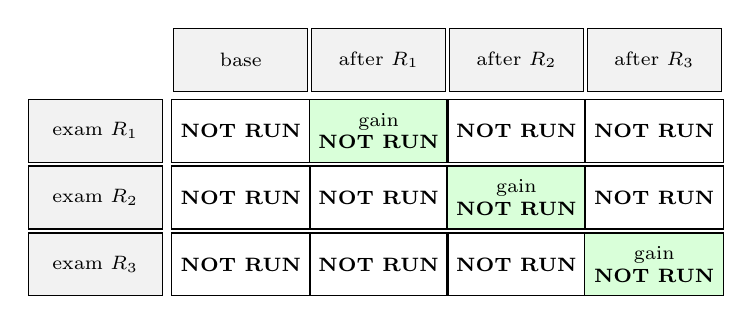
\begin{tikzpicture}[cell/.style={draw,minimum width=1.7cm,minimum height=0.8cm,font=\scriptsize,align=center}]
\foreach \c/\name in {0/base,1/after $R_1$,2/after $R_2$,3/after $R_3$}
  \node[cell,fill=gray!10] at (\c*1.75+1.85,0.9) {\name};
\foreach \r/\name in {0/exam $R_1$,1/exam $R_2$,2/exam $R_3$}
  \node[cell,fill=gray!10] at (0,-\r*0.85) {\name};
\foreach \r in {0,1,2}{
  \pgfmathtruncatemacro{\cc}{\r+1}
  \foreach \c in {0,1,2,3}{
    \ifnum\c=\cc
      \node[cell,fill=green!15] at (\c*1.75+1.85,-\r*0.85) {gain\\\notrun};
    \else
      \node[cell] at (\c*1.75+1.85,-\r*0.85) {\notrun};
    \fi
  }
}
\end{tikzpicture}
\caption{E3 result matrix. Shaded: the round that trained on that repository (the
primary gain). Cells to the right of a shaded cell test retention after later rounds; cells to its left
(including the base) test transfer and protocol learning. Nothing is measured yet.}\label{fig:matrix}
\end{figure}

\paragraph{What the test can decide.} \Cref{tab:design} and \cref{fig:power} give, for the
exact one-sided sign test, the discordant families needed and the power at assumed win
probabilities. With fewer than five non-tied families no decision is possible at
$\alpha=\alphalevel$, and a repository that yields fewer than about twenty reserved
families can reveal only large effects; such a result is reported as underpowered.
These are design calculations, not measurements.

\begin{table}[t]
\centering\small
\begin{tabular}{rrrrrr}
\toprule
Discordant & Wins needed & Smallest $p$ & \multicolumn{3}{c}{Power if $P(\text{win})=$} \\
clusters $n$ & for $p\le 0.05$ & (all wins) & 0.7 & 0.8 & 0.9 \\
\midrule
4 & none & 0.062 & 0.00 & 0.00 & 0.00 \\
5 & 5 & 0.031 & 0.17 & 0.33 & 0.59 \\
6 & 6 & 0.016 & 0.12 & 0.26 & 0.53 \\
8 & 7 & 0.0039 & 0.26 & 0.50 & 0.81 \\
10 & 9 & 0.00098 & 0.15 & 0.38 & 0.74 \\
15 & 12 & 3.1e-05 & 0.30 & 0.65 & 0.94 \\
20 & 15 & 9.5e-07 & 0.42 & 0.80 & 0.99 \\
30 & 20 & 9.3e-10 & 0.73 & 0.97 & 1.00 \\
\bottomrule
\end{tabular}

\caption{Exact one-sided sign test at $\alpha=\alphalevel$: wins required and power if each
non-tied family is a win with the stated probability (design calculation).}\label{tab:design}
\end{table}

\begin{figure}[t]
\centering
\begin{tikzpicture}
\begin{axis}[width=0.75\linewidth,height=5.2cm,xlabel={non-tied exam families $n$},
  ylabel={power},ymin=0,ymax=1.02,xmin=2,xmax=40,legend pos=south east,
  legend style={font=\scriptsize},grid=major,
  every axis plot/.append style={thick}]
\addplot[blue,mark=none] table[col sep=comma,x=n,y=q70] {generated/power_curve.csv};
\addplot[red!70!black,mark=none,dashed] table[col sep=comma,x=n,y=q80] {generated/power_curve.csv};
\addplot[green!50!black,mark=none,dotted] table[col sep=comma,x=n,y=q90] {generated/power_curve.csv};
\legend{$P(\text{win})=0.7$,$P(\text{win})=0.8$,$P(\text{win})=0.9$}
\end{axis}
\end{tikzpicture}
\caption{Power of the exact one-sided sign test ($\alpha=\alphalevel$) against the number of
non-tied families. The sawtooth is the discreteness of the test.}\label{fig:power}
\end{figure}

\paragraph{Leakage and contamination controls.} (i) Families are assigned before rollouts.
(ii) Hidden files are absent from the solver's tree; they are materialised only in the
verifier's directory. (iii) An exposure audit scans each trajectory for hidden paths, hidden
content shingles and the state-root path; an exposed experience fails with a counted reason
and is excluded from training and gates. (iv) The isolation level of each run
(\code{container} or \code{none}) is recorded; with \code{none} the audit detects but cannot
prevent. (v) Repositories that may be in the base model's pretraining data are flagged;
the base-arm comparison on the same exam bounds, but does not remove, that effect.

% SPDX-License-Identifier: CC-BY-4.0
% Copyright (c) 2026 Martin Schröder <info@swedishembedded.com>

\section{Audit of the existing stack against the protocol}\label{sec:audit}

Before building, we read the three code bases against the requirements of
\cref{sec:protocol}. The list below is what that reading found. These are
\emph{static findings}: each was located in source and none has yet been reproduced by a
failing test; an entry moves to a verified defect only when its regression test exists, and
the section is revised then.

\begin{enumerate}
\item \textbf{Loss masking of tool conversations.} The trainer's per-record masking
checks that each supervised span lies on a boundary of the rendered chat. Under the
Qwen3 template, an empty reasoning block is added to the last assistant turn only, so
non-final assistant turns of a multi-step conversation fail the boundary check; turns
with tool calls take that same path. Training on whole agent trajectories therefore needs
a per-answer prompt/completion encoding, with each completion equal to what the serving
renderer produces.
\item \textbf{Tool definitions lost between recording and training.} The agent records
the tool definitions of the run, but the trajectory-to-training projections we inspected
drop them, so a model would be trained on tool calls without the tool block it sees when
served. Splinter's projection also refuses a second user turn (the follow-up turns of the
solver) and substitutes its own system prompt.
\item \textbf{Trajectory fidelity in the agent SDK.} The exported trajectory has no marker
for a context compaction, lists every registered tool instead of the set offered in the
agent's mode, and turns unparseable tool-call arguments into an empty object. Each
changes what a training record would claim the model saw or did.
\item \textbf{Closed-book release probes.} The release gate's probes and serve check run
tasks closed-book; a suite of workspace tasks would be unmeasured and so fail the gate,
and text agreement between served and in-process answers is meaningless across
multi-step runs.
\item \textbf{Containment.} A coding agent's shell is not a sandbox; the file tools are
confined to a root but a command can read outside it. In the environment of this study the
container runtime and the user-namespace sandbox are both unusable, so runs have
isolation level \code{none}, and the exposure audit is detection, not prevention. A
previous coding loop also recorded a case in which a worker read a hidden test.
\item \textbf{Contamination paths.} A semantic-memory tool was not in the worker's
withheld set, and the agent runtime writes its audit log into the workspace.
\item \textbf{Serving.} Brain serves one adapter per process and selects it by manifest
digest; the manifest has a reader but no public writer.
\end{enumerate}

% SPDX-License-Identifier: CC-BY-4.0
% Copyright (c) 2026 Martin Schröder <info@swedishembedded.com>

\section{Results}\label{sec:results}

\Cref{tab:results} is generated from \code{data/results.csv}. A row exists only for a
finished run; an experiment without rows is printed \notrun. The number of measured rows in
this version is \measuredrows.

\begin{table}[t]
\centering\small
\begin{tabular}{llllrrrrl}
\toprule
Exp. & Repository & Round & Arm & Families & Wins & Losses & $p$ & Status \\
\midrule
E1 & \multicolumn{8}{l}{Plumbing: tools and masks reach the trainer (overfit test): \textbf{NOT RUN}} \\
E2 & \multicolumn{8}{l}{One repository: adapter against base on frozen exam families: \textbf{NOT RUN}} \\
E3 & \multicolumn{8}{l}{Sequential repositories: gain and retention across rounds: \textbf{NOT RUN}} \\
E4 & \multicolumn{8}{l}{Repository evolution: new revision, continued adapter: \textbf{NOT RUN}} \\
A1 & \multicolumn{8}{l}{Ablation: training on all trajectories, not only verified ones: \textbf{NOT RUN}} \\
A2 & \multicolumn{8}{l}{Ablation: no replay of earlier repositories: \textbf{NOT RUN}} \\
\bottomrule
\end{tabular}

\caption{Paired outcomes over exam-family clusters (wins: adapter resolves more of the
family than base; losses: fewer), with the exact one-sided sign test.}\label{tab:results}
\end{table}

No claim about learning is made in this version. The reader should conclude only that
the protocol is fixed (\cref{sec:protocol}), what it can decide (\cref{tab:design}),
and what must be repaired in the stack before the experiments can mean anything
(\cref{sec:audit}).

% SPDX-License-Identifier: CC-BY-4.0
% Copyright (c) 2026 Martin Schröder <info@swedishembedded.com>

\section{Discussion and limitations}

\paragraph{Alternative explanations a gain must survive.} A gain on a repository's
reserved families can come from (a) learning the repository, (b) learning the tool
protocol of the harness, (c) learning to undo the synthetic mutation operators rather
than to debug, or (d) memorisation of public code. E3's off-diagonal cells and A1 address
(a) against (b) and the value of verification; (c) is addressed only by adding
historical bug-fix tasks to the exam, which the mutation-seeded generator does not produce;
(d) is bounded, not removed, by comparing with the base on the same exam.

\paragraph{Limits.} One model size (a Qwen3 base of at most 8B parameters, set by what
trains and serves end to end on two 24~GB GPUs), one agent harness, Python fixtures first
with Rust repositories later because offline dependency vendoring needs a working
container backend, runs without process isolation in this environment, and exam sizes of
a single repository that may be too small for a significant sign test. Agent rollouts at
the lengths of real trajectories make training cost unmeasured for the 8B model until
the long-context cost is measured.

\paragraph{If the thesis fails.} A null on E2 with a working E1 means the pipeline runs and
does not help at these sample sizes and this data volume; it would be reported as
such, with the discordant counts, not as a defect of the idea.

\section{Conclusion}

We fixed a protocol for asking whether a local agent can be tuned to a repository,
repeatedly and cumulatively, without a person in the loop, stated what its primary test can
decide, and listed what had to be repaired in the stack first. We have not yet measured
whether it works.

% SPDX-License-Identifier: CC-BY-4.0
% Copyright (c) 2026 Martin Schröder <info@swedishembedded.com>

\section{Reproducibility}

\begin{itemize}
\item The PDF is built with \code{make papers/training-code-skills-with-splinter/pdf} from the
repository root (output \code{target/papers/training-code-skills-with-splinter.pdf}).
\item Every number in the tables comes from \code{data/results.csv} through
\code{scripts/build_data.py} (standard library only); the design table is computed, not
measured.
\item The frozen protocol is \code{prereg/protocol.md}. Each result row will add the
commands, commit hashes of Splinter, Sven and Brain, model checkpoint digest, harness
profile digest, seeds and hardware; no run commands exist yet, and none are claimed.
\item Hardware for the planned runs: two Tesla P40 (24~GB each).
\end{itemize}


\bibliographystyle{plainnat}
\bibliography{references}

\end{document}
